% REV00 Tue 04 May 2021 13:55:16 WIB
% START Tue 04 May 2021 13:55:16 WIB

\chapter{PODSNAPPERY}

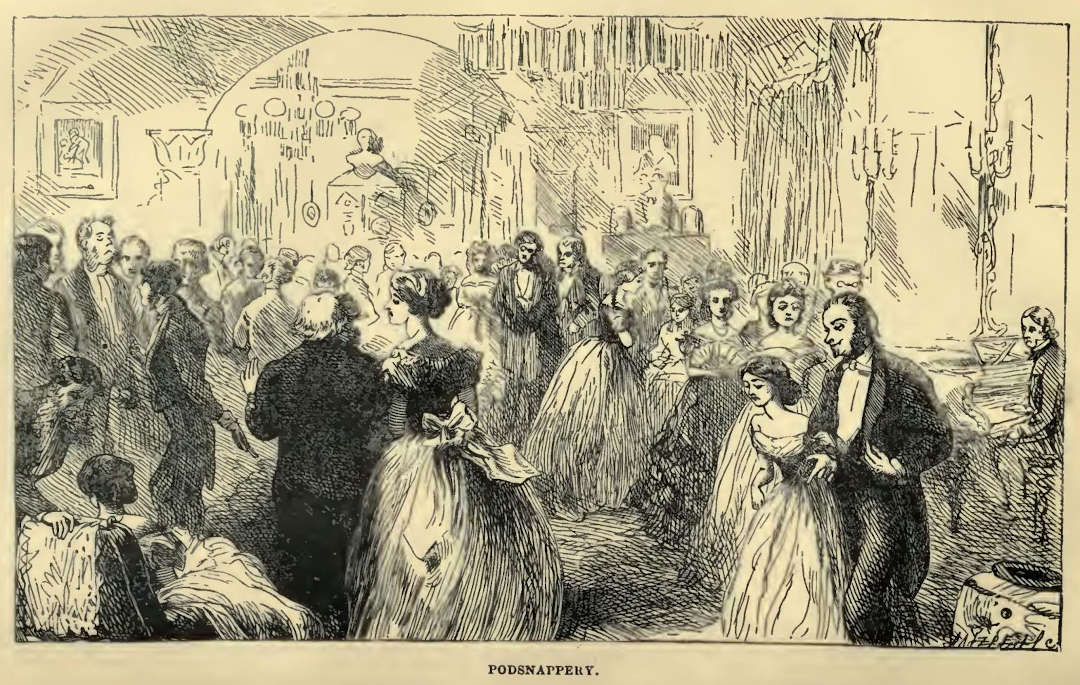
\includegraphics[scale=2.3]{01-11-01}

Mr Podsnap was well to do, and stood very high in Mr Podsnap’s opinion.
Beginning with a good inheritance, he had married a good inheritance,
and had thriven exceedingly in the Marine Insurance way, and was
quite satisfied. He never could make out why everybody was not quite
satisfied, and he felt conscious that he set a brilliant social example
in being particularly well satisfied with most things, and, above all
other things, with himself.

Thus happily acquainted with his own merit and importance, Mr Podsnap
settled that whatever he put behind him he put out of existence. There
was a dignified conclusiveness--not to add a grand convenience--in
this way of getting rid of disagreeables which had done much towards
establishing Mr Podsnap in his lofty place in Mr Podsnap’s satisfaction.
‘I don’t want to know about it; I don’t choose to discuss it; I don’t
admit it!’ Mr Podsnap had even acquired a peculiar flourish of his
right arm in often clearing the world of its most difficult problems, by
sweeping them behind him (and consequently sheer away) with those words
and a flushed face. For they affronted him.

Mr Podsnap’s world was not a very large world, morally; no, nor even
geographically: seeing that although his business was sustained upon
commerce with other countries, he considered other countries, with that
important reservation, a mistake, and of their manners and customs would
conclusively observe, ‘Not English!’ when, PRESTO! with a flourish of
the arm, and a flush of the face, they were swept away. Elsewise, the
world got up at eight, shaved close at a quarter-past, breakfasted at
nine, went to the City at ten, came home at half-past five, and dined
at seven. Mr Podsnap’s notions of the Arts in their integrity might have
been stated thus. Literature; large print, respectfully descriptive of
getting up at eight, shaving close at a quarter past, breakfasting
at nine, going to the City at ten, coming home at half-past five,
and dining at seven. Painting and Sculpture; models and portraits
representing Professors of getting up at eight, shaving close at a
quarter past, breakfasting at nine, going to the City at ten, coming
home at half-past five, and dining at seven. Music; a respectable
performance (without variations) on stringed and wind instruments,
sedately expressive of getting up at eight, shaving close at a quarter
past, breakfasting at nine, going to the City at ten, coming home at
half-past five, and dining at seven. Nothing else to be permitted to
those same vagrants the Arts, on pain of excommunication. Nothing else
To Be--anywhere!

As a so eminently respectable man, Mr Podsnap was sensible of its being
required of him to take Providence under his protection. Consequently he
always knew exactly what Providence meant. Inferior and less respectable
men might fall short of that mark, but Mr Podsnap was always up to it.
And it was very remarkable (and must have been very comfortable) that
what Providence meant, was invariably what Mr Podsnap meant.

These may be said to have been the articles of a faith and school
which the present chapter takes the liberty of calling, after its
representative man, Podsnappery. They were confined within close bounds,
as Mr Podsnap’s own head was confined by his shirt-collar; and they
were enunciated with a sounding pomp that smacked of the creaking of Mr
Podsnap’s own boots.

There was a Miss Podsnap. And this young rocking-horse was being trained
in her mother’s art of prancing in a stately manner without ever getting
on. But the high parental action was not yet imparted to her, and
in truth she was but an undersized damsel, with high shoulders, low
spirits, chilled elbows, and a rasped surface of nose, who seemed to
take occasional frosty peeps out of childhood into womanhood, and to
shrink back again, overcome by her mother’s head-dress and her father
from head to foot--crushed by the mere dead-weight of Podsnappery.

A certain institution in Mr Podsnap’s mind which he called ‘the young
person’ may be considered to have been embodied in Miss Podsnap, his
daughter. It was an inconvenient and exacting institution, as requiring
everything in the universe to be filed down and fitted to it. The
question about everything was, would it bring a blush into the cheek of
the young person? And the inconvenience of the young person was, that,
according to Mr Podsnap, she seemed always liable to burst into
blushes when there was no need at all. There appeared to be no line of
demarcation between the young person’s excessive innocence, and another
person’s guiltiest knowledge. Take Mr Podsnap’s word for it, and the
soberest tints of drab, white, lilac, and grey, were all flaming red to
this troublesome Bull of a young person.

The Podsnaps lived in a shady angle adjoining Portman Square. They were
a kind of people certain to dwell in the shade, wherever they dwelt.
Miss Podsnap’s life had been, from her first appearance on this planet,
altogether of a shady order; for, Mr Podsnap’s young person was likely
to get little good out of association with other young persons, and had
therefore been restricted to companionship with not very congenial older
persons, and with massive furniture. Miss Podsnap’s early views of life
being principally derived from the reflections of it in her father’s
boots, and in the walnut and rosewood tables of the dim drawing-rooms,
and in their swarthy giants of looking-glasses, were of a sombre cast;
and it was not wonderful that now, when she was on most days solemnly
tooled through the Park by the side of her mother in a great tall
custard-coloured phaeton, she showed above the apron of that vehicle
like a dejected young person sitting up in bed to take a startled look
at things in general, and very strongly desiring to get her head under
the counterpane again.

Said Mr Podsnap to Mrs Podsnap, ‘Georgiana is almost eighteen.’

Said Mrs Podsnap to Mr Podsnap, assenting, ‘Almost eighteen.’

Said Mr Podsnap then to Mrs Podsnap, ‘Really I think we should have some
people on Georgiana’s birthday.’

Said Mrs Podsnap then to Mr Podsnap, ‘Which will enable us to clear off
all those people who are due.’

So it came to pass that Mr and Mrs Podsnap requested the honour of the
company of seventeen friends of their souls at dinner; and that they
substituted other friends of their souls for such of the seventeen
original friends of their souls as deeply regretted that a prior
engagement prevented their having the honour of dining with Mr and Mrs
Podsnap, in pursuance of their kind invitation; and that Mrs Podsnap
said of all these inconsolable personages, as she checked them off with
a pencil in her list, ‘Asked, at any rate, and got rid of;’ and that
they successfully disposed of a good many friends of their souls in this
way, and felt their consciences much lightened.

There were still other friends of their souls who were not entitled to
be asked to dinner, but had a claim to be invited to come and take a
haunch of mutton vapour-bath at half-past nine. For the clearing off
of these worthies, Mrs Podsnap added a small and early evening to the
dinner, and looked in at the music-shop to bespeak a well-conducted
automaton to come and play quadrilles for a carpet dance.

Mr and Mrs Veneering, and Mr and Mrs Veneering’s bran-new bride and
bridegroom, were of the dinner company; but the Podsnap establishment
had nothing else in common with the Veneerings. Mr Podsnap could
tolerate taste in a mushroom man who stood in need of that sort
of thing, but was far above it himself. Hideous solidity was the
characteristic of the Podsnap plate. Everything was made to look as
heavy as it could, and to take up as much room as possible. Everything
said boastfully, ‘Here you have as much of me in my ugliness as if I
were only lead; but I am so many ounces of precious metal worth so much
an ounce;--wouldn’t you like to melt me down?’ A corpulent straddling
epergne, blotched all over as if it had broken out in an eruption rather
than been ornamented, delivered this address from an unsightly silver
platform in the centre of the table. Four silver wine-coolers, each
furnished with four staring heads, each head obtrusively carrying a big
silver ring in each of its ears, conveyed the sentiment up and down the
table, and handed it on to the pot-bellied silver salt-cellars. All the
big silver spoons and forks widened the mouths of the company expressly
for the purpose of thrusting the sentiment down their throats with every
morsel they ate.

The majority of the guests were like the plate, and included several
heavy articles weighing ever so much. But there was a foreign gentleman
among them: whom Mr Podsnap had invited after much debate with
himself--believing the whole European continent to be in mortal alliance
against the young person--and there was a droll disposition, not only on
the part of Mr Podsnap but of everybody else, to treat him as if he were
a child who was hard of hearing.

As a delicate concession to this unfortunately-born foreigner, Mr
Podsnap, in receiving him, had presented his wife as ‘Madame Podsnap;’
also his daughter as ‘Mademoiselle Podsnap,’ with some inclination to
add ‘ma fille,’ in which bold venture, however, he checked himself. The
Veneerings being at that time the only other arrivals, he had added (in
a condescendingly explanatory manner), ‘Monsieur Vey-nair-reeng,’ and
had then subsided into English.

‘How Do You Like London?’ Mr Podsnap now inquired from his station of
host, as if he were administering something in the nature of a powder or
potion to the deaf child; ‘London, Londres, London?’

The foreign gentleman admired it.

‘You find it Very Large?’ said Mr Podsnap, spaciously.

The foreign gentleman found it very large.

‘And Very Rich?’

The foreign gentleman found it, without doubt, enormement riche.

‘Enormously Rich, We say,’ returned Mr Podsnap, in a condescending
manner. ‘Our English adverbs do Not terminate in Mong, and We Pronounce
the “ch” as if there were a “t” before it. We say Ritch.’

‘Reetch,’ remarked the foreign gentleman.

‘And Do You Find, Sir,’ pursued Mr Podsnap, with dignity, ‘Many
Evidences that Strike You, of our British Constitution in the Streets Of
The World’s Metropolis, London, Londres, London?’

The foreign gentleman begged to be pardoned, but did not altogether
understand.

‘The Constitution Britannique,’ Mr Podsnap explained, as if he were
teaching in an infant school. ‘We Say British, But You Say Britannique,
You Know’ (forgivingly, as if that were not his fault). ‘The
Constitution, Sir.’

The foreign gentleman said, ‘Mais, yees; I know eem.’

A youngish sallowish gentleman in spectacles, with a lumpy forehead,
seated in a supplementary chair at a corner of the table, here caused
a profound sensation by saying, in a raised voice, ‘ESKER,’ and then
stopping dead.

‘Mais oui,’ said the foreign gentleman, turning towards him. ‘Est-ce
que? Quoi donc?’

But the gentleman with the lumpy forehead having for the time delivered
himself of all that he found behind his lumps, spake for the time no
more.

‘I Was Inquiring,’ said Mr Podsnap, resuming the thread of his
discourse, ‘Whether You Have Observed in our Streets as We should say,
Upon our Pavvy as You would say, any Tokens--’

The foreign gentleman, with patient courtesy entreated pardon; ‘But what
was tokenz?’

‘Marks,’ said Mr Podsnap; ‘Signs, you know, Appearances--Traces.’

‘Ah! Of a Orse?’ inquired the foreign gentleman.

‘We call it Horse,’ said Mr Podsnap, with forbearance. ‘In England,
Angleterre, England, We Aspirate the “H,” and We Say “Horse.” Only our
Lower Classes Say “Orse!”’

‘Pardon,’ said the foreign gentleman; ‘I am alwiz wrong!’

‘Our Language,’ said Mr Podsnap, with a gracious consciousness of being
always right, ‘is Difficult. Ours is a Copious Language, and Trying to
Strangers. I will not Pursue my Question.’

But the lumpy gentleman, unwilling to give it up, again madly said,
‘ESKER,’ and again spake no more.

‘It merely referred,’ Mr Podsnap explained, with a sense of meritorious
proprietorship, ‘to Our Constitution, Sir. We Englishmen are Very Proud
of our Constitution, Sir. It Was Bestowed Upon Us By Providence. No
Other Country is so Favoured as This Country.’

‘And ozer countries?--’ the foreign gentleman was beginning, when Mr
Podsnap put him right again.

‘We do not say Ozer; we say Other: the letters are “T” and “H;” You say
Tay and Aish, You Know; (still with clemency). The sound is “th”--“th!”’

‘And OTHER countries,’ said the foreign gentleman. ‘They do how?’

‘They do, Sir,’ returned Mr Podsnap, gravely shaking his head; ‘they
do--I am sorry to be obliged to say it--AS they do.’

‘It was a little particular of Providence,’ said the foreign gentleman,
laughing; ‘for the frontier is not large.’

‘Undoubtedly,’ assented Mr Podsnap; ‘But So it is. It was the Charter
of the Land. This Island was Blest, Sir, to the Direct Exclusion of
such Other Countries as--as there may happen to be. And if we were all
Englishmen present, I would say,’ added Mr Podsnap, looking round upon
his compatriots, and sounding solemnly with his theme, ‘that there is in
the Englishman a combination of qualities, a modesty, an independence,
a responsibility, a repose, combined with an absence of everything
calculated to call a blush into the cheek of a young person, which one
would seek in vain among the Nations of the Earth.’

Having delivered this little summary, Mr Podsnap’s face flushed, as he
thought of the remote possibility of its being at all qualified by
any prejudiced citizen of any other country; and, with his favourite
right-arm flourish, he put the rest of Europe and the whole of Asia,
Africa, and America nowhere.

The audience were much edified by this passage of words; and Mr Podsnap,
feeling that he was in rather remarkable force to-day, became smiling
and conversational.

‘Has anything more been heard, Veneering,’ he inquired, ‘of the lucky
legatee?’

‘Nothing more,’ returned Veneering, ‘than that he has come into
possession of the property. I am told people now call him The Golden
Dustman. I mentioned to you some time ago, I think, that the young lady
whose intended husband was murdered is daughter to a clerk of mine?’

‘Yes, you told me that,’ said Podsnap; ‘and by-the-bye, I wish you would
tell it again here, for it’s a curious coincidence--curious that the
first news of the discovery should have been brought straight to your
table (when I was there), and curious that one of your people should
have been so nearly interested in it. Just relate that, will you?’

Veneering was more than ready to do it, for he had prospered exceedingly
upon the Harmon Murder, and had turned the social distinction it
conferred upon him to the account of making several dozen of bran-new
bosom-friends. Indeed, such another lucky hit would almost have set him
up in that way to his satisfaction. So, addressing himself to the most
desirable of his neighbours, while Mrs Veneering secured the next most
desirable, he plunged into the case, and emerged from it twenty minutes
afterwards with a Bank Director in his arms. In the mean time, Mrs
Veneering had dived into the same waters for a wealthy Ship-Broker, and
had brought him up, safe and sound, by the hair. Then Mrs Veneering had
to relate, to a larger circle, how she had been to see the girl, and how
she was really pretty, and (considering her station) presentable.
And this she did with such a successful display of her eight aquiline
fingers and their encircling jewels, that she happily laid hold of a
drifting General Officer, his wife and daughter, and not only restored
their animation which had become suspended, but made them lively friends
within an hour.

Although Mr Podsnap would in a general way have highly disapproved of
Bodies in rivers as ineligible topics with reference to the cheek of the
young person, he had, as one may say, a share in this affair which made
him a part proprietor. As its returns were immediate, too, in the way
of restraining the company from speechless contemplation of the
wine-coolers, it paid, and he was satisfied.

And now the haunch of mutton vapour-bath having received a gamey
infusion, and a few last touches of sweets and coffee, was quite ready,
and the bathers came; but not before the discreet automaton had got
behind the bars of the piano music-desk, and there presented the
appearance of a captive languishing in a rose-wood jail. And who now
so pleasant or so well assorted as Mr and Mrs Alfred Lammle, he all
sparkle, she all gracious contentment, both at occasional intervals
exchanging looks like partners at cards who played a game against All
England.

There was not much youth among the bathers, but there was no youth
(the young person always excepted) in the articles of Podsnappery. Bald
bathers folded their arms and talked to Mr Podsnap on the hearthrug;
sleek-whiskered bathers, with hats in their hands, lunged at Mrs Podsnap
and retreated; prowling bathers, went about looking into ornamental
boxes and bowls as if they had suspicions of larceny on the part of the
Podsnaps, and expected to find something they had lost at the bottom;
bathers of the gentler sex sat silently comparing ivory shoulders. All
this time and always, poor little Miss Podsnap, whose tiny efforts (if
she had made any) were swallowed up in the magnificence of her mother’s
rocking, kept herself as much out of sight and mind as she could,
and appeared to be counting on many dismal returns of the day. It was
somehow understood, as a secret article in the state proprieties of
Podsnappery that nothing must be said about the day. Consequently this
young damsel’s nativity was hushed up and looked over, as if it were
agreed on all hands that it would have been better that she had never
been born.

The Lammles were so fond of the dear Veneerings that they could not for
some time detach themselves from those excellent friends; but at length,
either a very open smile on Mr Lammle’s part, or a very secret elevation
of one of his gingerous eyebrows--certainly the one or the other--seemed
to say to Mrs Lammle, ‘Why don’t you play?’ And so, looking about her,
she saw Miss Podsnap, and seeming to say responsively, ‘That card?’ and
to be answered, ‘Yes,’ went and sat beside Miss Podsnap.

Mrs Lammle was overjoyed to escape into a corner for a little quiet
talk.

It promised to be a very quiet talk, for Miss Podsnap replied in a
flutter, ‘Oh! Indeed, it’s very kind of you, but I am afraid I DON’T
talk.’

‘Let us make a beginning,’ said the insinuating Mrs Lammle, with her
best smile.

‘Oh! I am afraid you’ll find me very dull. But Ma talks!’

That was plainly to be seen, for Ma was talking then at her usual
canter, with arched head and mane, opened eyes and nostrils.

‘Fond of reading perhaps?’

‘Yes. At least I--don’t mind that so much,’ returned Miss Podsnap.

‘M-m-m-m-music.’ So insinuating was Mrs Lammle that she got half a dozen
ms into the word before she got it out.

‘I haven’t nerve to play even if I could. Ma plays.’

(At exactly the same canter, and with a certain flourishing appearance
of doing something, Ma did, in fact, occasionally take a rock upon the
instrument.)

‘Of course you like dancing?’

‘Oh no, I don’t,’ said Miss Podsnap.

‘No? With your youth and attractions? Truly, my dear, you surprise me!’

‘I can’t say,’ observed Miss Podsnap, after hesitating considerably, and
stealing several timid looks at Mrs Lammle’s carefully arranged face,
‘how I might have liked it if I had been a--you won’t mention it, WILL
you?’

‘My dear! Never!’

‘No, I am sure you won’t. I can’t say then how I should have liked it,
if I had been a chimney-sweep on May-day.’

‘Gracious!’ was the exclamation which amazement elicited from Mrs
Lammle.

‘There! I knew you’d wonder. But you won’t mention it, will you?’

‘Upon my word, my love,’ said Mrs Lammle, ‘you make me ten times more
desirous, now I talk to you, to know you well than I was when I sat over
yonder looking at you. How I wish we could be real friends! Try me as a
real friend. Come! Don’t fancy me a frumpy old married woman, my dear;
I was married but the other day, you know; I am dressed as a bride now,
you see. About the chimney-sweeps?’

‘Hush! Ma’ll hear.’

‘She can’t hear from where she sits.’

‘Don’t you be too sure of that,’ said Miss Podsnap, in a lower voice.
‘Well, what I mean is, that they seem to enjoy it.’

‘And that perhaps you would have enjoyed it, if you had been one of
them?’

Miss Podsnap nodded significantly.

‘Then you don’t enjoy it now?’

‘How is it possible?’ said Miss Podsnap. ‘Oh it is such a dreadful
thing! If I was wicked enough--and strong enough--to kill anybody, it
should be my partner.’

This was such an entirely new view of the Terpsichorean art as
socially practised, that Mrs Lammle looked at her young friend in some
astonishment. Her young friend sat nervously twiddling her fingers in
a pinioned attitude, as if she were trying to hide her elbows. But this
latter Utopian object (in short sleeves) always appeared to be the great
inoffensive aim of her existence.

‘It sounds horrid, don’t it?’ said Miss Podsnap, with a penitential
face.

Mrs Lammle, not very well knowing what to answer, resolved herself into
a look of smiling encouragement.

‘But it is, and it always has been,’ pursued Miss Podsnap, ‘such a trial
to me! I so dread being awful. And it is so awful! No one knows what
I suffered at Madame Sauteuse’s, where I learnt to dance and make
presentation-curtseys, and other dreadful things--or at least where they
tried to teach me. Ma can do it.’

‘At any rate, my love,’ said Mrs Lammle, soothingly, ‘that’s over.’

‘Yes, it’s over,’ returned Miss Podsnap, ‘but there’s nothing gained by
that. It’s worse here, than at Madame Sauteuse’s. Ma was there, and Ma’s
here; but Pa wasn’t there, and company wasn’t there, and there were not
real partners there. Oh there’s Ma speaking to the man at the piano! Oh
there’s Ma going up to somebody! Oh I know she’s going to bring him
to me! Oh please don’t, please don’t, please don’t! Oh keep away, keep
away, keep away!’ These pious ejaculations Miss Podsnap uttered with her
eyes closed, and her head leaning back against the wall.

But the Ogre advanced under the pilotage of Ma, and Ma said, ‘Georgiana,
Mr Grompus,’ and the Ogre clutched his victim and bore her off to his
castle in the top couple. Then the discreet automaton who had surveyed
his ground, played a blossomless tuneless ‘set,’ and sixteen disciples
of Podsnappery went through the figures of - 1, Getting up at eight and
shaving close at a quarter past - 2, Breakfasting at nine - 3, Going to
the City at ten - 4, Coming home at half-past five - 5, Dining at seven,
and the grand chain.

While these solemnities were in progress, Mr Alfred Lammle (most loving
of husbands) approached the chair of Mrs Alfred Lammle (most loving of
wives), and bending over the back of it, trifled for some few seconds
with Mrs Lammle’s bracelet. Slightly in contrast with this brief airy
toying, one might have noticed a certain dark attention in Mrs Lammle’s
face as she said some words with her eyes on Mr Lammle’s waistcoat, and
seemed in return to receive some lesson. But it was all done as a breath
passes from a mirror.

And now, the grand chain riveted to the last link, the discreet
automaton ceased, and the sixteen, two and two, took a walk among
the furniture. And herein the unconsciousness of the Ogre Grompus was
pleasantly conspicuous; for, that complacent monster, believing that
he was giving Miss Podsnap a treat, prolonged to the utmost stretch
of possibility a peripatetic account of an archery meeting; while his
victim, heading the procession of sixteen as it slowly circled about,
like a revolving funeral, never raised her eyes except once to steal a
glance at Mrs Lammle, expressive of intense despair.

At length the procession was dissolved by the violent arrival of a
nutmeg, before which the drawing-room door bounced open as if it were a
cannon-ball; and while that fragrant article, dispersed through several
glasses of coloured warm water, was going the round of society, Miss
Podsnap returned to her seat by her new friend.

‘Oh my goodness,’ said Miss Podsnap. ‘THAT’S over! I hope you didn’t
look at me.’

‘My dear, why not?’

‘Oh I know all about myself,’ said Miss Podsnap.

‘I’ll tell you something I know about you, my dear,’ returned Mrs Lammle
in her winning way, ‘and that is, you are most unnecessarily shy.’

‘Ma ain’t,’ said Miss Podsnap. ‘--I detest you! Go along!’ This shot
was levelled under her breath at the gallant Grompus for bestowing an
insinuating smile upon her in passing.

‘Pardon me if I scarcely see, my dear Miss Podsnap,’ Mrs Lammle was
beginning when the young lady interposed.

‘If we are going to be real friends (and I suppose we are, for you are
the only person who ever proposed it) don’t let us be awful. It’s awful
enough to BE Miss Podsnap, without being called so. Call me Georgiana.’

‘Dearest Georgiana,’ Mrs Lammle began again.

‘Thank you,’ said Miss Podsnap.

‘Dearest Georgiana, pardon me if I scarcely see, my love, why your
mamma’s not being shy, is a reason why you should be.’

‘Don’t you really see that?’ asked Miss Podsnap, plucking at her fingers
in a troubled manner, and furtively casting her eyes now on Mrs Lammle,
now on the ground. ‘Then perhaps it isn’t?’

‘My dearest Georgiana, you defer much too readily to my poor opinion.
Indeed it is not even an opinion, darling, for it is only a confession
of my dullness.’

‘Oh YOU are not dull,’ returned Miss Podsnap. ‘I am dull, but you
couldn’t have made me talk if you were.’

Some little touch of conscience answering this perception of her having
gained a purpose, called bloom enough into Mrs Lammle’s face to make it
look brighter as she sat smiling her best smile on her dear Georgiana,
and shaking her head with an affectionate playfulness. Not that it meant
anything, but that Georgiana seemed to like it.

‘What I mean is,’ pursued Georgiana, ‘that Ma being so endowed with
awfulness, and Pa being so endowed with awfulness, and there being
so much awfulness everywhere--I mean, at least, everywhere where I
am--perhaps it makes me who am so deficient in awfulness, and frightened
at it--I say it very badly--I don’t know whether you can understand what
I mean?’

‘Perfectly, dearest Georgiana!’ Mrs Lammle was proceeding with every
reassuring wile, when the head of that young lady suddenly went back
against the wall again and her eyes closed.

‘Oh there’s Ma being awful with somebody with a glass in his eye! Oh I
know she’s going to bring him here! Oh don’t bring him, don’t bring him!
Oh he’ll be my partner with his glass in his eye! Oh what shall I do!’
This time Georgiana accompanied her ejaculations with taps of her feet
upon the floor, and was altogether in quite a desperate condition. But,
there was no escape from the majestic Mrs Podsnap’s production of an
ambling stranger, with one eye screwed up into extinction and the other
framed and glazed, who, having looked down out of that organ, as if he
descried Miss Podsnap at the bottom of some perpendicular shaft, brought
her to the surface, and ambled off with her. And then the captive at the
piano played another ‘set,’ expressive of his mournful aspirations after
freedom, and other sixteen went through the former melancholy motions,
and the ambler took Miss Podsnap for a furniture walk, as if he had
struck out an entirely original conception.

In the mean time a stray personage of a meek demeanour, who had wandered
to the hearthrug and got among the heads of tribes assembled there in
conference with Mr Podsnap, eliminated Mr Podsnap’s flush and
flourish by a highly unpolite remark; no less than a reference to the
circumstance that some half-dozen people had lately died in the streets,
of starvation. It was clearly ill-timed after dinner. It was not adapted
to the cheek of the young person. It was not in good taste.

‘I don’t believe it,’ said Mr Podsnap, putting it behind him.

The meek man was afraid we must take it as proved, because there were
the Inquests and the Registrar’s returns.

‘Then it was their own fault,’ said Mr Podsnap.

Veneering and other elders of tribes commended this way out of it. At
once a short cut and a broad road.

The man of meek demeanour intimated that truly it would seem from
the facts, as if starvation had been forced upon the culprits in
question--as if, in their wretched manner, they had made their weak
protests against it--as if they would have taken the liberty of staving
it off if they could--as if they would rather not have been starved upon
the whole, if perfectly agreeable to all parties.

‘There is not,’ said Mr Podsnap, flushing angrily, ‘there is not a
country in the world, sir, where so noble a provision is made for the
poor as in this country.’

The meek man was quite willing to concede that, but perhaps it
rendered the matter even worse, as showing that there must be something
appallingly wrong somewhere.

‘Where?’ said Mr Podsnap.

The meek man hinted Wouldn’t it be well to try, very seriously, to find
out where?

‘Ah!’ said Mr Podsnap. ‘Easy to say somewhere; not so easy to say
where! But I see what you are driving at. I knew it from the first.
Centralization. No. Never with my consent. Not English.’

An approving murmur arose from the heads of tribes; as saying, ‘There
you have him! Hold him!’

He was not aware (the meek man submitted of himself) that he was driving
at any ization. He had no favourite ization that he knew of. But he
certainly was more staggered by these terrible occurrences than he was
by names, of howsoever so many syllables. Might he ask, was dying of
destitution and neglect necessarily English?

‘You know what the population of London is, I suppose,’ said Mr Podsnap.

The meek man supposed he did, but supposed that had absolutely nothing
to do with it, if its laws were well administered.

‘And you know; at least I hope you know;’ said Mr Podsnap, with
severity, ‘that Providence has declared that you shall have the poor
always with you?’

The meek man also hoped he knew that.

‘I am glad to hear it,’ said Mr Podsnap with a portentous air. ‘I am
glad to hear it. It will render you cautious how you fly in the face of
Providence.’

In reference to that absurd and irreverent conventional phrase, the meek
man said, for which Mr Podsnap was not responsible, he the meek man had
no fear of doing anything so impossible; but--

But Mr Podsnap felt that the time had come for flushing and flourishing
this meek man down for good. So he said:

‘I must decline to pursue this painful discussion. It is not pleasant to
my feelings; it is repugnant to my feelings. I have said that I do not
admit these things. I have also said that if they do occur (not that I
admit it), the fault lies with the sufferers themselves. It is not for
ME’--Mr Podsnap pointed ‘me’ forcibly, as adding by implication though
it may be all very well for YOU--‘it is not for me to impugn the
workings of Providence. I know better than that, I trust, and I have
mentioned what the intentions of Providence are. Besides,’ said
Mr Podsnap, flushing high up among his hair-brushes, with a strong
consciousness of personal affront, ‘the subject is a very disagreeable
one. I will go so far as to say it is an odious one. It is not one to be
introduced among our wives and young persons, and I--’ He finished with
that flourish of his arm which added more expressively than any words,
And I remove it from the face of the earth.

Simultaneously with this quenching of the meek man’s ineffectual fire;
Georgiana having left the ambler up a lane of sofa, in a No Thoroughfare
of back drawing-room, to find his own way out, came back to Mrs Lammle.
And who should be with Mrs Lammle, but Mr Lammle. So fond of her!

‘Alfred, my love, here is my friend. Georgiana, dearest girl, you must
like my husband next to me.’

Mr Lammle was proud to be so soon distinguished by this special
commendation to Miss Podsnap’s favour. But if Mr Lammle were prone to be
jealous of his dear Sophronia’s friendships, he would be jealous of her
feeling towards Miss Podsnap.

‘Say Georgiana, darling,’ interposed his wife.

‘Towards--shall I?--Georgiana.’ Mr Lammle uttered the name, with a
delicate curve of his right hand, from his lips outward. ‘For never have
I known Sophronia (who is not apt to take sudden likings) so attracted
and so captivated as she is by--shall I once more?--Georgiana.’

The object of this homage sat uneasily enough in receipt of it, and then
said, turning to Mrs Lammle, much embarrassed:

‘I wonder what you like me for! I am sure I can’t think.’

‘Dearest Georgiana, for yourself. For your difference from all around
you.’

‘Well! That may be. For I think I like you for your difference from all
around me,’ said Georgiana with a smile of relief.

‘We must be going with the rest,’ observed Mrs Lammle, rising with a
show of unwillingness, amidst a general dispersal. ‘We are real friends,
Georgiana dear?’

‘Real.’

‘Good night, dear girl!’

She had established an attraction over the shrinking nature upon which
her smiling eyes were fixed, for Georgiana held her hand while she
answered in a secret and half-frightened tone:

‘Don’t forget me when you are gone away. And come again soon. Good
night!’

Charming to see Mr and Mrs Lammle taking leave so gracefully, and going
down the stairs so lovingly and sweetly. Not quite so charming to see
their smiling faces fall and brood as they dropped moodily into separate
corners of their little carriage. But to be sure that was a sight behind
the scenes, which nobody saw, and which nobody was meant to see.

Certain big, heavy vehicles, built on the model of the Podsnap plate,
took away the heavy articles of guests weighing ever so much; and the
less valuable articles got away after their various manners; and the
Podsnap plate was put to bed. As Mr Podsnap stood with his back to the
drawing-room fire, pulling up his shirtcollar, like a veritable cock
of the walk literally pluming himself in the midst of his possessions,
nothing would have astonished him more than an intimation that Miss
Podsnap, or any other young person properly born and bred, could not be
exactly put away like the plate, brought out like the plate, polished
like the plate, counted, weighed, and valued like the plate. That such
a young person could possibly have a morbid vacancy in the heart for
anything younger than the plate, or less monotonous than the plate;
or that such a young person’s thoughts could try to scale the region
bounded on the north, south, east, and west, by the plate; was a
monstrous imagination which he would on the spot have flourished into
space. This perhaps in some sort arose from Mr Podsnap’s blushing young
person being, so to speak, all cheek; whereas there is a possibility
that there may be young persons of a rather more complex organization.

If Mr Podsnap, pulling up his shirt-collar, could only have heard
himself called ‘that fellow’ in a certain short dialogue, which passed
between Mr and Mrs Lammle in their opposite corners of their little
carriage, rolling home!

‘Sophronia, are you awake?’

‘Am I likely to be asleep, sir?’

‘Very likely, I should think, after that fellow’s company. Attend to
what I am going to say.’

‘I have attended to what you have already said, have I not? What else
have I been doing all to-night.’

‘Attend, I tell you,’ (in a raised voice) ‘to what I am going to say.
Keep close to that idiot girl. Keep her under your thumb. You have her
fast, and you are not to let her go. Do you hear?’

‘I hear you.’

‘I foresee there is money to be made out of this, besides taking that
fellow down a peg. We owe each other money, you know.’

Mrs Lammle winced a little at the reminder, but only enough to shake her
scents and essences anew into the atmosphere of the little carriage, as
she settled herself afresh in her own dark corner.


